\documentclass{article}
\usepackage[T2A]{fontenc}
\usepackage[utf8]{inputenc}
\usepackage[russian]{babel}
\usepackage[margin=2cm]{geometry}
\usepackage{icomma}
\usepackage{amsmath}
\usepackage{amssymb}
\usepackage{enumitem}
\usepackage{graphicx}
\usepackage{url}

\pagestyle{empty}

\begin{document}

% ==============================================================================

\begin{flushright}
    \textit{Выполнил: Максимов Н. Д.} \\
    \textit{Группа: 09-414} \\
    \textit{Вариант: 8}
\end{flushright}

\begin{center}
    \bfseries\LARGE Отчет по лабораторной работе №2
\end{center}
\bigskip

% ==============================================================================

\section*{Задание 1.0}
По заданию необходимо проверить однородность (равенство дисперсий) двух выборок из нормального распределения по одновыборочному критерию Стьюдента (двухвыборочный вариант) при уровне значимости $\alpha=0,025$.

\paragraph{Гипотезы}
\begin{itemize}[nosep]
    \item $H_0$: Средние значения равны ($\mu_1 = \mu_2$);
    \item $H_1$: Средние отличаются ($\mu_1 \neq \mu_2$).
\end{itemize}
Согласно алгоритму проверки по двухвыборочному варианту критерия Стьюдента средние разности выборок будет сравниваться с нулем.

\paragraph{Расчетные формулы} Для двусторонней критической области, соответствующей $H_1$, критическая константа и $p$-значение вычисляются как
\[ C_\text{крит} = F_\text{stud}^{-1} \Big(1-\frac\alpha2 ~\Big|~ n-1\Big) \qquad\qquad p\text{-value} = 2(1-F_\text{stud}(|t| ~|~ n-1)), \]
где $F$ --- распределению Стьюдента, $t$ --- статистика критерия, а $n$ --- число степеней свободы выборок.

\paragraph{Результаты вычислений} ~\vspace{-0.5\baselineskip}
\[ t = -0,183 \qquad\qquad C_\text{крит} = 2,311 \qquad\qquad p\text{-value} = 0,855 \]

\paragraph{Вывод} Так как $p\text{-value} = 0,855 > \alpha = 0,025$ (или $|t| < C_{\text{крит}}$), статистических оснований для отклонения нулевой гипотезы нет. Выборки можно считать однородными.

% ==============================================================================

\section*{Задание 1}
По заданию необходимо сравнить дисперсии двух независимых выборок из нормального распределения по критерию Фишера при уровне значимости $\alpha = 0,025$.

\paragraph{Гипотезы}
\begin{itemize}[nosep]
    \item $H_0$: Дисперсии двух групп равны ($\sigma_1^2 = \sigma_2^2$);
    \item $H_1$: Дисперсия первой группы меньше ($\sigma_1^2 < \sigma_2^2$).
\end{itemize}

\paragraph{Расчетные формулы} Для левосторонней критической области, соответствующей $H_1$, критическая константа и $p$-значение вычисляются как
\[ C_{\text{крит}} = F^{-1}(\alpha ~|~ k_1, k_2) \qquad\qquad p\text{-value} = F(f ~|~ k_1, k_2), \]
где $F$ --- распределению Фишера, $f$ --- статистика критерия, а $k_1$ и $k_2$ --- числа степеней свободы двух выборок.

\paragraph{Результаты вычислений} ~\vspace{-0.5\baselineskip}
\[ f = 0,903 \qquad\qquad C_{\text{крит}} = 0,612 \qquad\qquad p\text{-value} = 0,342 \]

\paragraph{Вывод} Так как $p\text{-value} = 0,342 > \alpha = 0,025$ (или $f > C_{\text{крит}}$), статистических оснований для отклонения нулевой гипотезы нет. Дисперсии двух выборок можно считать равными.

% ==============================================================================

\section*{Задание 2}
Используя критерий Колмогорова, проверить, что функция распределения выборочных данных совпадает с экспоненциальным распределением с заданной интенсивностью ($\mathbb{E}(\lambda=2)$) при уровне значимости $\alpha = 0,01$.

\paragraph{Гипотезы}
\begin{itemize}[nosep]
    \item $H_0$: Распределение совпадает с экспоненциальным ($F \sim \mathbb{E}(\lambda=2)$);
    \item $H_1$: Распределение не совпадает с экспоненциальным.
\end{itemize}

\paragraph{Расчетные формулы} Для критерия Колмогорова критическая области всегда является правосторонней, критическая константа и $p$-значения вычисляются как
\[ C_\text{крит} = F^{-1}(1 - \alpha) \qquad\qquad p\text{-value} = 1-F(\sqrt{n} \cdot D_n), \]
где $F$ --- распределение Колмогорова, $D_n$ --- супремум-статистика критерия, $n$ --- размер выборки.

\paragraph{Результаты вычислений} ~\vspace{-0.5\baselineskip}
\[ D_n = 0,151 \qquad\qquad C_\text{крит} = 1,628 \qquad\qquad p\text{-value} = 0,107 \]

\paragraph{Вывод} Так как $p\text{-value} = 0,107 > \alpha = 0,01$ (или $\sqrt{n} \cdot D_n < C_{\text{крит}}$), статистических оснований для отклонения нулевой гипотезы нет. Функцию распределения выборки можно считать экспоненциальной с интенсивностью 2, что подтверждается графически.
\begin{center}
    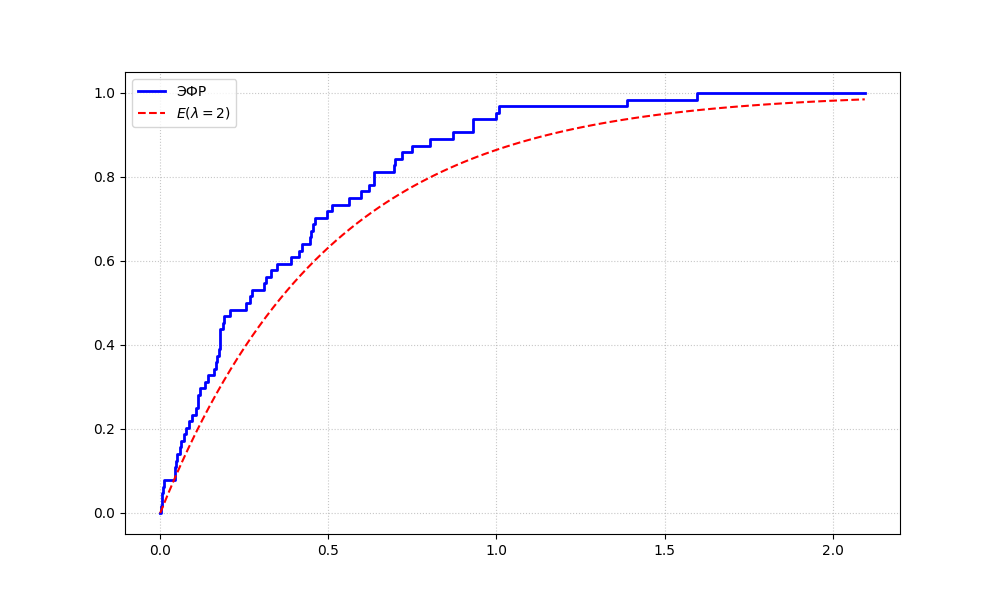
\includegraphics[scale=0.5]{image.png}
\end{center}

% ==============================================================================

\vfill
\noindent\rule{\textwidth}{0.4pt}
\small Полный исходный код лабораторной работы доступен в репозитории на GitHub: \url{https://github.com/mndkpfu/MS}

% ==============================================================================

\end{document}